\documentclass[a4paper,10pt,twocolumn,uplatex]{jsarticle}
\usepackage{style/nislab,style/resume}

%---------------------------------------------------------------------
% レジュメ種別・日付設定(要変更)
% \type{} 1:修士論文諮問会 2:卒業論文発表会 3:月例発表会 4:研究室合同発表会
%---------------------------------------------------------------------
\type{4}
\year{2022}
\month{9}
\date{5}

%---------------------------------------------------------------------
% ページ番号設定(要変更)
%---------------------------------------------------------------------
\setcounter{page}{1}

%---------------------------------------------------------------------
% 変更不要
%---------------------------------------------------------------------
\begin{document}

%---------------------------------------------------------------------
% タイトル作成部分(要変更)
% \maketitle{タイトル}{title}{名前}{name}
%---------------------------------------------------------------------
\maketitle{狭小空間監視のための複数ドローンを利用した\\ 動的な三次元環境地図生成によるAR可視化手法}
{AR Visualization Method by Dynamic 3D Environmental Map Generation\\ Using Multiple Drones for Narrow Space Surveillance}
{竹内 一真}
{Kazuma Takeuchi}

% --------------------------- Section1  ---------------------------

\section{はじめに}
近年,多方面でのドローンを活用した事業が登場しており,インフラ点検や災害調査など,応用分野を拡大しながら,ドローン用途は急速に成長し,熟練された操縦者に限らず,より多くの人がドローンを使用する機会が増加している\cite{Nonami}.
中でも小型ドローンの特徴である機体の大きさを活かして,人間が入れないような狭い空間での活躍の場も増加しており,将来的には狭小空間の未知領域探査への応用が期待されている.
しかし,小型ドローンはセンサ搭載制限があるため,障害物回避の支援がないことが多く,衝突の危険性があり,
また,障害物回避の機能を搭載していても,狭小空間では障害物回避が行えない場面が多く存在する\cite{syohou}.
そのため,ドローン搭載のカメラ映像を頼りにした手動による操縦を必要とする.
しかし,狭小空間でのドローン飛行は遮蔽物が多く,操縦者は遮られた視点からの操縦を必要とするため,死角領域内のドローン操縦では,ドローンを視認できない中,衝突することなく,安全に操縦する技術が求められる.
% オンボードカメラ搭載ドローンを使用する場合では,操縦者は,ドローンから送られる空撮した映像を元に操縦が可能となる.
% しかし,カメラが前方しか写さないことにより,前方以外の死角が多くなり,状況認識が不十分となるため\cite{Green},狭小空間のように狭く,障害物が多いような環境では,操縦は困難である.

\par
そこで,Augmented Reality(AR)を用いて死角領域内を可視化することにより,狭小空間での未知領域探査におけるドローンの操縦性向上や安全性向上が期待されている\cite{Erat}.
事前に走行環境をマッピングすることで三次元環境地図を取得し,空間認識を提供している.
しかし,狭小空間のドローン操縦において,事前に三次元環境地図を用意することは困難なため,
実際の未知領域探査において,ドローンが一からマッピング,自己位置推定などを行う環境でも同じ効果を発揮できるのか示されていない.
また,ドローンはバッテリー上限が短く,短時間での効率的な探査を必要とする中で\cite{Gupta},一台のドローンのみで探査を行うには多くの時間を要すため,複数ドローンの利用が検討されている.
関連研究では一台のドローンのみを想定していたが,複数ドローンを適応する場合,各ドローンのセンサ情報を共有できるシステムが必要である.
% しかし,各ドローンの位置情報や探査領域を把握できないことによる衝突危険性や探査済み領域の再探査の非効率性が考えられるため,各ドローンのセンサ情報を共有できるシステムが必要である.
本研究では,狭小空間における死角領域内おいて,複数ドローンによる衝突危険性の軽減,効率的な未知領域探査を実現するため,各ドローンのセンサ情報を統合した上で,ARにより操縦者の死角領域内を可視化するシステムを開発する.

% --------------------------- Figure  ---------------------------

\begin{figure}[!tb]
  \centering
  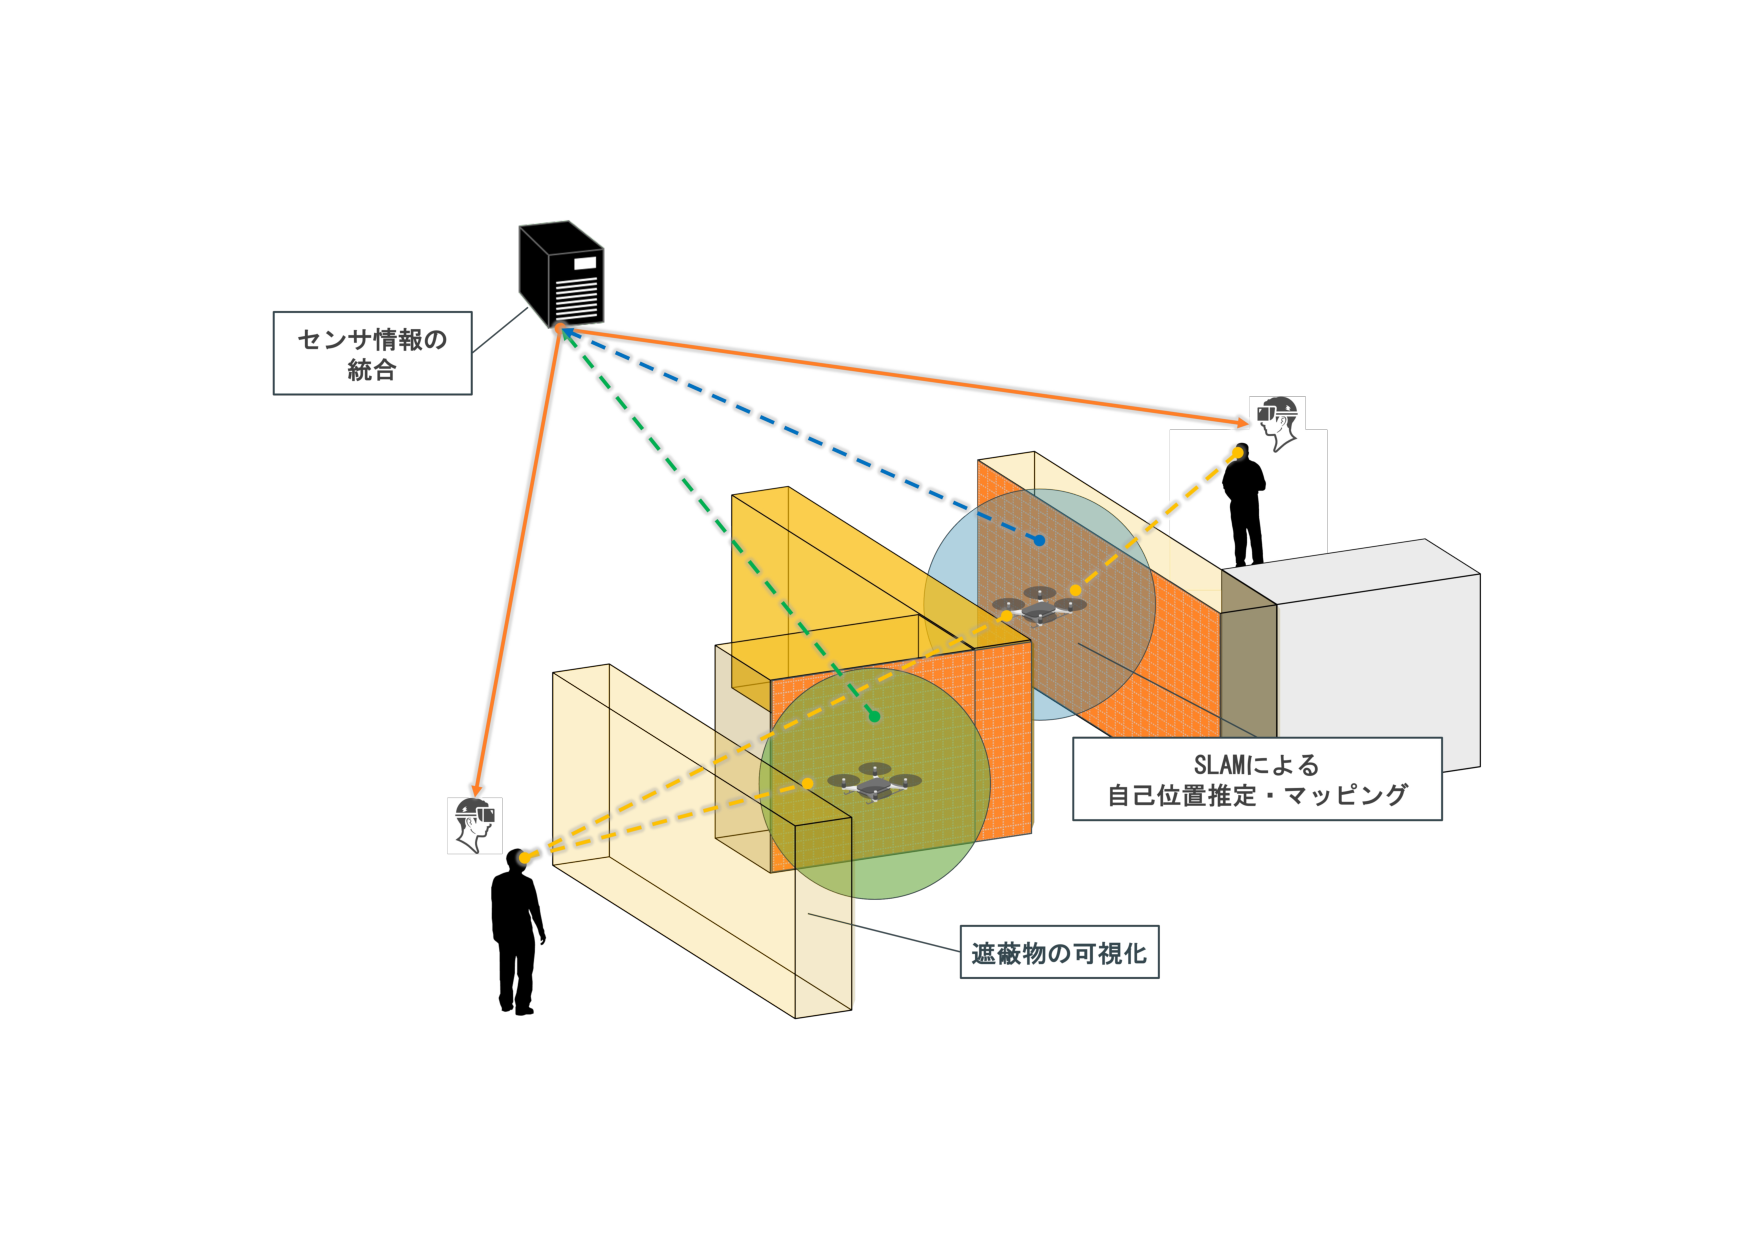
\includegraphics[width=\linewidth]{img/outline.pdf}
  \caption{複数ドローン混在時における死角領域内の可視化}
  \label{fig:outline}
\end{figure}


% --------------------------- Section2  ---------------------------

\section{提案システム}
\subsection{概要}
本研究では,狭小空間により,操縦者と小型ドローン(以下,ドローン)の間に遮蔽物があり,ドローンを視認できない環境を「死角領域」とする.
提案システムを図\ref{fig:outline}に示しており,各ドローンがリアルタイムで走行環境をマッピングし生成された三次元環境地図
を,ARにより重畳表示することで,死角領域内の空間認識を提供している.
\par

\subsection{死角領域内のAR可視化}
先に述べた関連研究\cite{Erat}を元に,操縦者に死角領域内の空間認識を提供する.
ドローンと操縦者の間に遮蔽物が存在する場合,ドローンが飛行している場所が操縦者にとっての死角領域となる.
死角領域が存在すると判断したとき,マッピングした三次元環境地図における遮蔽物を透過した上で,現実環境に重畳表示することで,仮想的に死角領域の空間認識を提供する.
操縦者は,死角領域内を飛行するドローンを視認することはできないが,ARによって仮想のドローンと,ドローン周辺の三次元環境を視認することができる.

\subsection{複数ドローンのセンサ情報統合}
本研究におけるドローン操縦では,リアルタイムでマッピングを行い,三次元環境地図を作成する必要がある.
そこで,各ドローンはVisual SLAMであるORB-SLAM2を用いて,単眼カメラで取得した画像から特徴点を抽出し,自己位置推定を行い,
周囲の環境の点群情報を取得する.
また,各ドローンの位置情報,生成した点群情報は個々で独立している.
そこで,各ドローンをワールド座標系で管理し,各ドローンの位置情報,点群情報を統合し,操縦者へ提供する仮想的な三次元環境地図,ドローンを生成する.
% また,三次元環境地図はセンサーデータの重ね合わせによって生成しており,膨大な数の点の集合であり,
% データ量が非常に大きいため,点群情報をダウンサンプリングすることでデータ量を削減している.
生成した三次元環境地図を操縦者へ提供し,三次元環境地図上の遮蔽物を透過することで死角領域内を可視化する.
しかし,透過した遮蔽物が重なることで,ドローンに最も近傍の遮蔽物,障害物がどこに位置するか認識できなくなることが考えられる.
そのため,ドローンから距離の遠い遮蔽物の透明度を向上し,ドローンから距離の近い遮蔽物の透明度を低下することにより,ドローン周辺の遮蔽物,障害物を強調表示し,操縦者目線では認識が困難な物体の形状を把握できるか検証する.
これにより,遮蔽物の重なりの可視化による情報過多を防いでいる.

% --------------------------- Figure  ---------------------------

\begin{figure}[!tb]
  \centering
  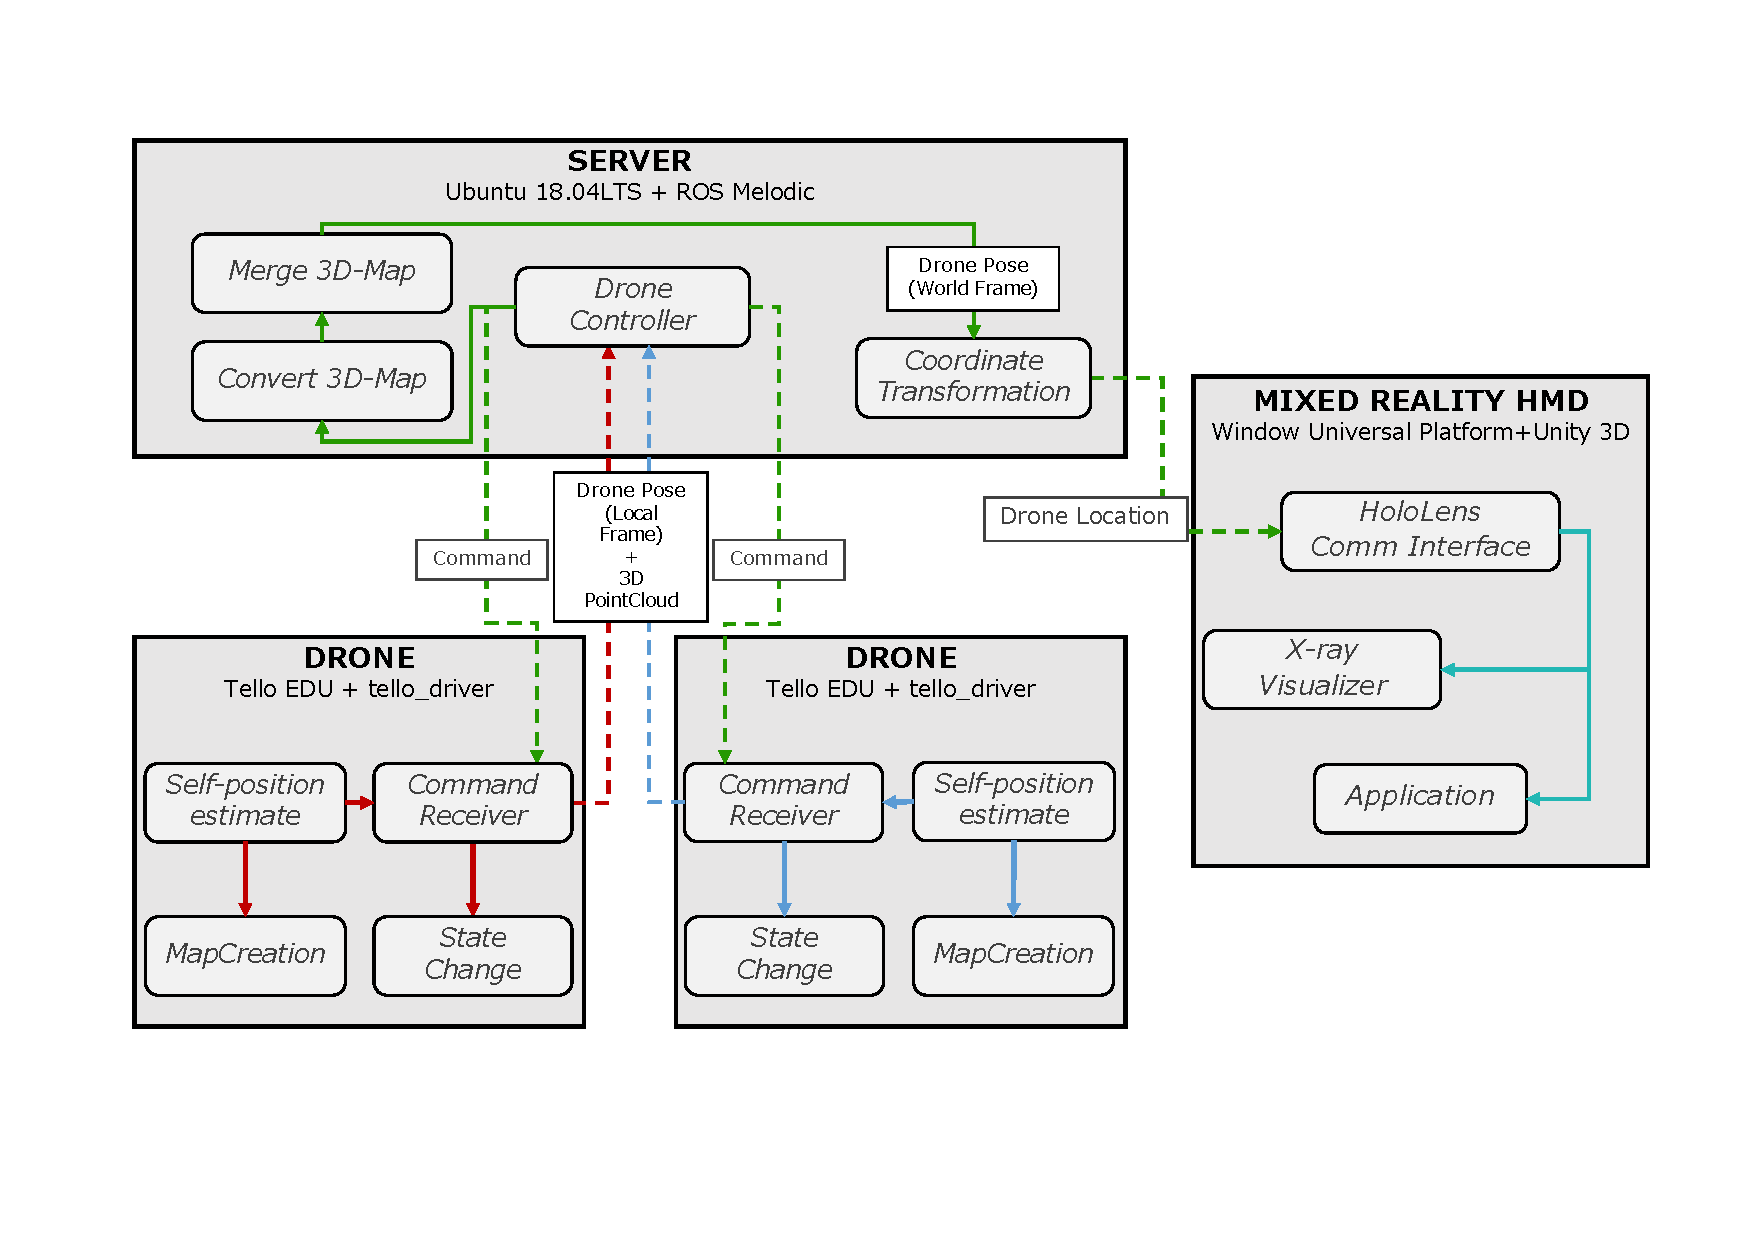
\includegraphics[width=\linewidth]{img/system.pdf}
  \caption{システム構成}
  \label{fig:system}
\end{figure}
  
% --------------------------- Section3  ---------------------------

\section{評価}

\subsection{実装環境}
システム構成を図\ref{fig:system}に示す.
使用するドローンはRyze Tech社製Tello EDU(以下,Tello)を用いる.Telloはプログラミングによってフライトコントロールを行うことができ,
規定のコマンドを送信することで飛行制御することができる.
\par
ARHMDはMicrosoft HoloLens2(以下,HoloLens)を使用する.
作成した三次元環境地図を,ゲーム・アニメーションエンジンであるUnity内の3D仮想空間上に配置し,操縦者の位置情報と,Unity内の三次元環境地図の位置合わせを行うことで,空間認識を提供する.
\par
サーバではTello,HoloLensとUDP通信を行なっており,常時,Telloの傾きや移動距離をHoloLensに送信する.
Telloより受け取った値をUnity 座標系へ変換し,変換後の値を反映させることにより,仮想ドローンの位置合わせを行なっている.
% ここでUDPを使用する理由として,Tello,サーバ,HoloLens間の遅延低減を目的とする.

\subsection{実験}
提案システムのドローン操縦への影響を評価するため,実験協力者による実験を行う.
実験協力者は狭小空間における未知領域をドローンにより探査し,与えられた地点まで飛行し,停止するタスクを繰り返し行う.
実験では従来のドローンのカメラ映像をもとに飛行する操縦手法,死角領域内を可視化した操縦手法,複数ドローンのセンサ情報を統合した操縦手法の計3つの手法で実験を行う.



\subsection{評価項目}
本提案手法を用いることによって狭小空間探査を手軽に安全に行え
るかを検証するため,主観的評価と客観的評価を行う.主観的評価として参加者へのアンケート,
客観的評価として操縦者がタスクを完了するまでの平均操縦時間,障害物への平均衝突回数,ドローン移動コマンドの平均間隔時間を評価する.

% --------------------------- Section4  ---------------------------

\section{おわりに}

小型ドローンは機体の大きさを活かして,インフラ点検や災害調査のような,人間が立ち入れない狭小空間での活躍が増えている.
しかし,狭小空間でのドローン飛行では,遮蔽物による視点が遮られる死角領域内での操縦を必要とする.
% また,従来の操縦法では状況認識が不十分であるため,ドローン周辺に位置する障害物が多い狭小空間では,ドローン操縦は困難である.
そのため,遮蔽物,障害物が多い狭小空間では,死角領域内におけるドローン飛行の危険性を軽減する必要がある.
\par
そこで本研究では,各ドローンがリアルタイムで飛行環境をマッピングし生成された三次元環境地図をもとに,ARにより操縦者の死角領域内に存在するドローンと周辺環境を可視化するARシステムを提案する.
本提案システムについて,死角領域内でのドローン操縦性,探査時間の効率性を評価実験する.

%---------------------------------------------------------------------
% Bibliography(参考文献)
%---------------------------------------------------------------------
% thebibliography を利用する場合は以下を使用
\footnotesize{
  \begin{thebibliography}{99}
    \bibitem{Nonami}
    野波健蔵:ドローン技術の現状と課題およびビジネス最前,情報管理,Vol.59,No.11,pp.755-763(2017).
    
    \bibitem{syohou}
    山越靖之,木田哲夫,湯浅弘章:屋内空間におけるドローンの活用に関する検証 (平成 30 年度消防技術安全所の検証成果等) – (消防活動・隊員の安全管理に関する技術改良・検証),消防技術安全所報, No. 56, pp. 26–37 (2019).
    
    \bibitem{Erat}
    Erat, O., Isop, W. A., Kalkofen, D. and Schmalstieg,D.: Application of UAV imaging platform for vegeta-tion analysis based on spectral-spatial methods, {\it IEEE Transactions on Visualization and Computer Graphics}, Vol. 24, No. 4, pp. 1437-1446 (2018).
    
    \bibitem{Gupta}
    Gupta, L., Jain, R. and Vaszkun, G.: Survey of Im-portant Issues in UAV Communication Networks, IEEE Communications Surveys \& Tutorials, Vol. 18, No. 2,pp. 1123-1152 (2016).
    
  \end{thebibliography}
}

% BibTex を利用する場合は以下を使用(初めての人には難しいかも)
% \bibliographystyle{junsrt}
% \bibliography{myref}

%---------------------------------------------------------------------
\end{document}
%---------------------------------------------------------------------